\section{Requirements and Message Protocol}
\label{sec:protocol}

\begin{guidance}[Requirements and message protocol (15 marks)]
Describe and diagram your \textbf{final} protocol: physical link (interface,
baud rate, frame format), \textbf{framing} (terminator, maximum frame length,
timeout), \textbf{board encoding}, the complete \textbf{command set}, and
\textbf{every response and error}. Cover new game, move, win/draw and
disconnect. Include at least one \textbf{sequence diagram}. \textbf{Highlight
every departure} from the brief's reference protocol (p.~3) and justify each
one. A reader should be able to write a compatible client from this section
alone.
\end{guidance}

\subsection{Physical Layer and Framing: Lines of at Most 64 Bytes Frame the Stream}
Communication between the PC client and the STM32F051 microcontroller occurs over a full-duplex asynchronous serial link via the \texttt{USART1} peripheral, utilizing pins \texttt{PA9} (\texttt{TX}) and \texttt{PA10} (\texttt{RX}). Signals are routed through the on-board ST-LINK Virtual COM Port (VCP) at 115200 baud with 8 data bits, no parity bit, and 1 stop bit (8N1). No hardware flow control is used.

Messages consist of printable 7-bit ASCII characters (\texttt{0x20}--\texttt{0x7E}) framed by a line-feed terminator (\texttt{\textbackslash n}, \texttt{0x0A}). To accommodate operating system and terminal differences, carriage-return characters (\texttt{\textbackslash r}, \texttt{0x0D}) are filtered upon ingestion. Input framing rules, bounds, and fault-recovery behaviours are summarized in Table~\ref{tab:framing}. The receive buffer is constrained to $\text{MAX\_FRAME\_LEN} = 64$ bytes; exceeding this limit flushes the index to zero to avoid stack corruption. To handle truncated transmissions without deadlock, an inter-byte silence timer clears partial buffers if no new bytes arrive within $\text{FRAME\_TIMEOUT} = 500\,\text{ms}$.

\begin{table}[t]
\centering
\caption{Framing rules, bounds, and fault responses.}
\label{tab:framing}
\footnotesize
\begin{tabular}{@{}L{2.8cm}L{5.2cm}@{}}
\toprule
Rule & Server Behaviour \\
\midrule
Frame Terminator & \texttt{\textbackslash n} (\texttt{0x0A}) completes frame, null-terminates string, and flags \texttt{frame\_ready = 1}. \\
Carriage Return & \texttt{\textbackslash r} (\texttt{0x0D}) is silently discarded during ingestion. \\
Max Frame Length & 64 bytes. Buffer overflow resets write index to 0 without corrupting memory. \\
Incomplete Frame & Inter-byte silence timeout (500\,ms) discards partial buffers and resets index to 0. \\
Invalid Characters & Non-ASCII or malformed headers trigger an immediate \texttt{NACK: BADCMD}. \\
\bottomrule
\end{tabular}
\end{table}

\subsection{Board and Fleet Coordinate Encoding}
The Battleship grid is configured as a $10 \times 10$ matrix with columns labeled A--J ($x \in [0, 9]$) and rows labeled 1--10 ($y \in [0, 9]$). A single coordinate is encoded as \texttt{<Col><Row>} (e.g.\ \texttt{A1}, \texttt{F7}, \texttt{J10}). Standard fleets comprise 5 orthogonal ships: Carrier (\texttt{C}, length 5), Battleship (\texttt{B}, length 4), Destroyer (\texttt{D}, length 3), Submarine (\texttt{S}, length 3), and Patrol Boat (\texttt{P}, length 2).

Fleet deployments are encoded as a canonical sequence of 10 coordinate endpoints representing the starting and ending cells of each ship in order of decreasing length:
\begin{align}
\label{eq:fleet_str}
\text{\texttt{FLEET: }} \langle P\rangle,&\langle C_S\rangle,\langle C_E\rangle,\langle B_S\rangle,\langle B_E\rangle, \nonumber\\
&\langle D_S\rangle,\langle D_E\rangle,\langle S_S\rangle,\langle S_E\rangle,\langle P_S\rangle,\langle P_E\rangle
\end{align}
For example, the deployment string \texttt{FLEET:~1,A1,A5,} \texttt{B1,B4,C1,C3,} \texttt{D1,D3,E1,E2} deploys Player~1's Carrier from A1 to A5, Battleship from B1 to B4, Destroyer from C1 to C3, Submarine from D1 to D3, and Patrol Boat from E1 to E2. 

Internally, each grid cell is stored as a single byte. Bits $0\text{x}00$--$0\text{x}05$ store the assigned \texttt{ShipType} (where 0 represents unhit water), and bit $0\text{x}80$ acts as the targeted mask. During active gameplay, board state is never broadcast in full to prevent client-side inspection. Instead, localized events (\texttt{HIT}, \texttt{MISS}, \texttt{SUNK}) are streamed, and the full layout is only retrievable post-match via \texttt{STATUS: <P>,<coords...>} to expose enemy positions on the game-over screen.

\begin{table}[t]
\centering
\caption{Command set and accepted states ($^\dagger$denotes extension).}
\label{tab:commands}
\scriptsize
\begin{tabular}{@{}L{2.2cm}L{1.9cm}L{3.9cm}@{}}
\toprule
Request & Accepted in State & Success Response \\
\midrule
\texttt{CONNECT} & Any & \texttt{OK} \\
\texttt{NEW: PVP}$^\dagger$ & \texttt{IDLE}, \texttt{GAME\_OVER} & \texttt{OK: NEW\_PVP} \\
\texttt{NEW: AI}$^\dagger$ & \texttt{IDLE}, \texttt{GAME\_OVER} & \texttt{OK: NEW\_AI} \\
\texttt{FLEET: <p>,<c>}$^\dagger$ & \texttt{SETUP} & \texttt{OK: SETUP\_P2} (P1 in PVP) \newline \texttt{OK: IN\_PROGRESS} (P2/AI) \\
\texttt{SHOOT: <p>,<xy>} & \texttt{IN\_PROGRESS} & \texttt{MISS: <opp>,<xy>} \newline \texttt{HIT: <opp>,<xy>} \newline \texttt{SUNK: <opp>,<s>,<xy1>,<xy2>} \newline \texttt{WIN: <p>,<s>,<xy1>,<xy2>} \\
\texttt{STATE: <p>} & \texttt{GAME\_OVER} & \texttt{STATUS: <p>,<fleet\_coords...>} \\
\texttt{DISCONNECT} & Any & \texttt{OK} \\
\bottomrule
\end{tabular}
\end{table}

\subsection{Command Set and Asynchronous Notifications}
Table~\ref{tab:commands} lists the complete set of accepted client commands. State transitions are strictly governed by the embedded FSM:
\begin{itemize}
    \item \textbf{\texttt{CONNECT}} / \textbf{\texttt{DISCONNECT}}: Resets internal variables, halts LED blinking, and establishes an active session in \texttt{STATE\_IDLE}.
    \item \textbf{\texttt{NEW: PVP}} / \textbf{\texttt{NEW: AI}}: Clears previous grid buffers and initiates fleet deployment (\texttt{STATE\_SETUP}). \texttt{NEW: AI} additionally seeds the pseudo-random generator via \texttt{HAL\_GetTick() $\oplus$ SysTick->VAL}.
    \item \textbf{\texttt{FLEET}}: Validates all 5 ships in temporary storage. If valid, locks the placement into memory. In AI mode, the microcontroller immediately deploys its own fleet and advances to \texttt{STATE\_IN\_PROGRESS}.
    \item \textbf{\texttt{SHOOT}}: Evaluates target coordinates. If valid, the target cell is marked, turn counters update, and health is adjusted. In AI mode, the MCU immediately executes a counter-attack and appends its response.
    \item \textbf{Asynchronous Hardware Reset}: Pressing the on-board user button (\texttt{PA0}) triggers a debounced interrupt, returns the server to \texttt{STATE\_IDLE}, and transmits \texttt{EVENT: RESET} to force the GUI client to the main menu.
\end{itemize}

\subsection{Error Responses and Strict Validation Precedence}
The server follows a deterministic, hierarchical error evaluation sequence for every incoming command, ensuring predictable responses:
\begin{enumerate}
    \item \textbf{Framing Check}: Overlength frames and framing timeouts clear the buffer without generating a reply.
    \item \textbf{Syntax and Parameter Parsing}: Malformed command strings, missing delimiters, out-of-range player IDs ($\ne 1, 2$), or unparseable coordinate tokens fail parsing and yield \texttt{NACK: BADCMD}.
    \item \textbf{State Machine Feasibility}: Commands sent during an inappropriate state (e.g.\ \texttt{SHOOT} before fleet deployment) yield \texttt{NACK: NOGAME} or \texttt{NACK: OUT\_OF\_STATE,<state>}.
    \item \textbf{Turn Enforcement}: Commands submitted by the inactive player yield \texttt{NACK: NOTURN}.
    \item \textbf{Geometry and Bounds Checks}: Ship placements that are diagonal, out-of-grid, or mismatched in length yield \texttt{NACK: BADCOORDS,<ship>}.
    \item \textbf{Overlap and Duplicate Checks}: Ship placements colliding with existing vessels yield \texttt{NACK: OCCUPIED,<ship>,<overlap>}. Targeted shots hitting an already-fired cell yield \texttt{NACK: REPEAT}.
\end{enumerate}
Table~\ref{tab:errors} outlines every error code and its state invariant guarantee.

\begin{table}[t]
\centering
\caption{Error responses, emission criteria, and state guarantees.}
\label{tab:errors}
\footnotesize
\begin{tabular}{@{}L{2.6cm}L{5.4cm}@{}}
\toprule
Error Response & Trigger Condition and State Guarantee \\
\midrule
\texttt{NACK: BADCMD} & Header unrecognised or parameters syntactically invalid. State unmodified. \\
\texttt{NACK: NOGAME} & Action received while in \texttt{STATE\_IDLE}. State unmodified. \\
\texttt{NACK: OUT\_OF\_STATE} & Command not permitted in current FSM phase (e.g.\ firing in setup). State unmodified. \\
\texttt{NACK: NOTURN} & Player ID does not match \texttt{current\_turn}. Turn remains with active player. \\
\texttt{NACK: BADCOORDS} & Ship is diagonal, off-board, or wrong length; or shot out-of-bounds. State unmodified. \\
\texttt{NACK: OCCUPIED} & Ship placement overlaps an already positioned ship. Entire fleet placement aborted. \\
\texttt{NACK: REPEAT} & Target cell already fired upon (bit $0\text{x}80$ set). Turn is preserved. \\
\bottomrule
\end{tabular}
\end{table}

\subsection{Departures from the Reference Protocol}
Several justified departures from the brief's Tic-Tac-Toe reference protocol (brief, p.~3) were implemented:
\begin{itemize}
    \item \textbf{Event-Based Outcomes vs.\ Board Broadcasting}: The reference protocol returns the entire board state on each move (\texttt{OK:BOARD:<chars>}). In Battleship, transmitting both grids would defeat the game's hidden-information premise. The server instead emits targeted events (\texttt{HIT}, \texttt{MISS}, \texttt{SUNK}), and only exposes the opponent's grid upon match completion.
    \item \textbf{Dedicated Setup Phase (\texttt{STATE\_SETUP})}: Battleship requires deploying multi-cell fleets prior to combat. The \texttt{FLEET} command performs atomic validation of all 5 ships before entering combat.
    \item \textbf{Diagnostic Rejection Codes}: Generic rejections were extended with contextual tokens (e.g.\ \texttt{NACK: OCCUPIED,C,B} identifies Carrier-Battleship overlap; \texttt{NACK: REPEAT} flags re-fired cells), enabling rich GUI feedback.
    \item \textbf{Absence of Draws}: In sequential Battleship with 17 finite ship cells across a $10 \times 10$ grid, fleet annihilation guarantees a definitive victor, making \texttt{DRAW} unreachable.
\end{itemize}

\begin{figure}[t]
\centering
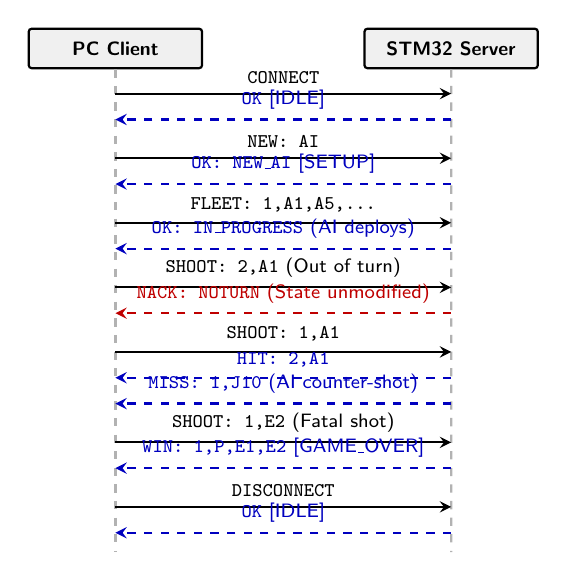
\begin{tikzpicture}[
    scale=0.82, every node/.style={font=\scriptsize\sffamily},
    lifeline/.style={thick, dashed, gray!60},
    msg/.style={->, >=stealth, thick},
    reply/.style={->, >=stealth, thick, dashed, blue!75!black},
    nack/.style={->, >=stealth, thick, dashed, red!75!black},
    box/.style={draw, thick, fill=gray!12, rounded corners=1pt, minimum width=2.2cm, minimum height=0.5cm}
]
    % Entities
    \node[box] (cli) at (0, 0) {\textbf{PC Client}};
    \node[box] (stm) at (5.2, 0) {\textbf{STM32 Server}};
    
    % Lifelines
    \draw[lifeline] (cli) -- (0, -7.8);
    \draw[lifeline] (stm) -- (5.2, -7.8);
    
    % Messages
    \draw[msg] (0, -0.7) -- node[above] {\texttt{CONNECT}} (5.2, -0.7);
    \draw[reply] (5.2, -1.1) -- node[above] {\texttt{OK} [IDLE]} (0, -1.1);
    
    \draw[msg] (0, -1.7) -- node[above] {\texttt{NEW: AI}} (5.2, -1.7);
    \draw[reply] (5.2, -2.1) -- node[above] {\texttt{OK: NEW\_AI} [SETUP]} (0, -2.1);
    
    \draw[msg] (0, -2.7) -- node[above] {\texttt{FLEET: 1,A1,A5,...}} (5.2, -2.7);
    \draw[reply] (5.2, -3.1) -- node[above] {\texttt{OK: IN\_PROGRESS} (AI deploys)} (0, -3.1);
    
    % Rejected Move
    \draw[msg] (0, -3.7) -- node[above] {\texttt{SHOOT: 2,A1} (Out of turn)} (5.2, -3.7);
    \draw[nack] (5.2, -4.1) -- node[above] {\textbf{\texttt{NACK: NOTURN}} (State unmodified)} (0, -4.1);
    
    % Combat Exchange
    \draw[msg] (0, -4.7) -- node[above] {\texttt{SHOOT: 1,A1}} (5.2, -4.7);
    \draw[reply] (5.2, -5.1) -- node[above] {\texttt{HIT: 2,A1}} (0, -5.1);
    \draw[reply] (5.2, -5.5) -- node[above] {\texttt{MISS: 1,J10} (AI counter-shot)} (0, -5.5);
    
    % Terminal Shot
    \draw[msg] (0, -6.1) -- node[above] {\texttt{SHOOT: 1,E2} (Fatal shot)} (5.2, -6.1);
    \draw[reply] (5.2, -6.5) -- node[above] {\texttt{WIN: 1,P,E1,E2} [GAME\_OVER]} (0, -6.5);
    
    % Teardown
    \draw[msg] (0, -7.1) -- node[above] {\texttt{DISCONNECT}} (5.2, -7.1);
    \draw[reply] (5.2, -7.5) -- node[above] {\texttt{OK} [IDLE]} (0, -7.5);
\end{tikzpicture}
\caption{Protocol sequence diagram showing connection, fleet deployment, out-of-turn rejection, combat exchange with AI retaliation, and terminal win resolution.}
\label{fig:sequence}
\end{figure}
